\chapter{\diva\divaspace general theory\label{chaptheory}}
\vspace*{-2cm}
\lettrine[lines=2, loversize=-0.1, lraise=0.1]{T}{his} chapter is dedicated to the description of the theoretical background necessary to understand how the \diva\, software works. As only the main ideas are summarized, the reader is invited to refer to the articles mentioned in the bibliography.

\minitoc


\section{The gridding problem\label{gridding}}
%----------------------------------------------

In oceanography a typical concern consists in determining a field $\varphi(\mathbf{r})$ on a regular grid of positions $\mathbf{r}$, knowing $N_{d}$ data in locations $\mathbf{r_{j}}, j=1,\ldots, N_{d}$. This is called the \textit{gridding problem} (Fig. \ref{gridproblem}) and is useful for many applications such as data analysis, graphical display, forcing or initialization of a model.

In this chapter we consider only two-dimensional cases, but generalization can be done to $3D$ and even $4$D (using "distance" in time, but being aware of autocorrelations as in seasonal signals).

\begin{figure}[htpb]
	\centering
	\parbox{.5\textwidth}{
		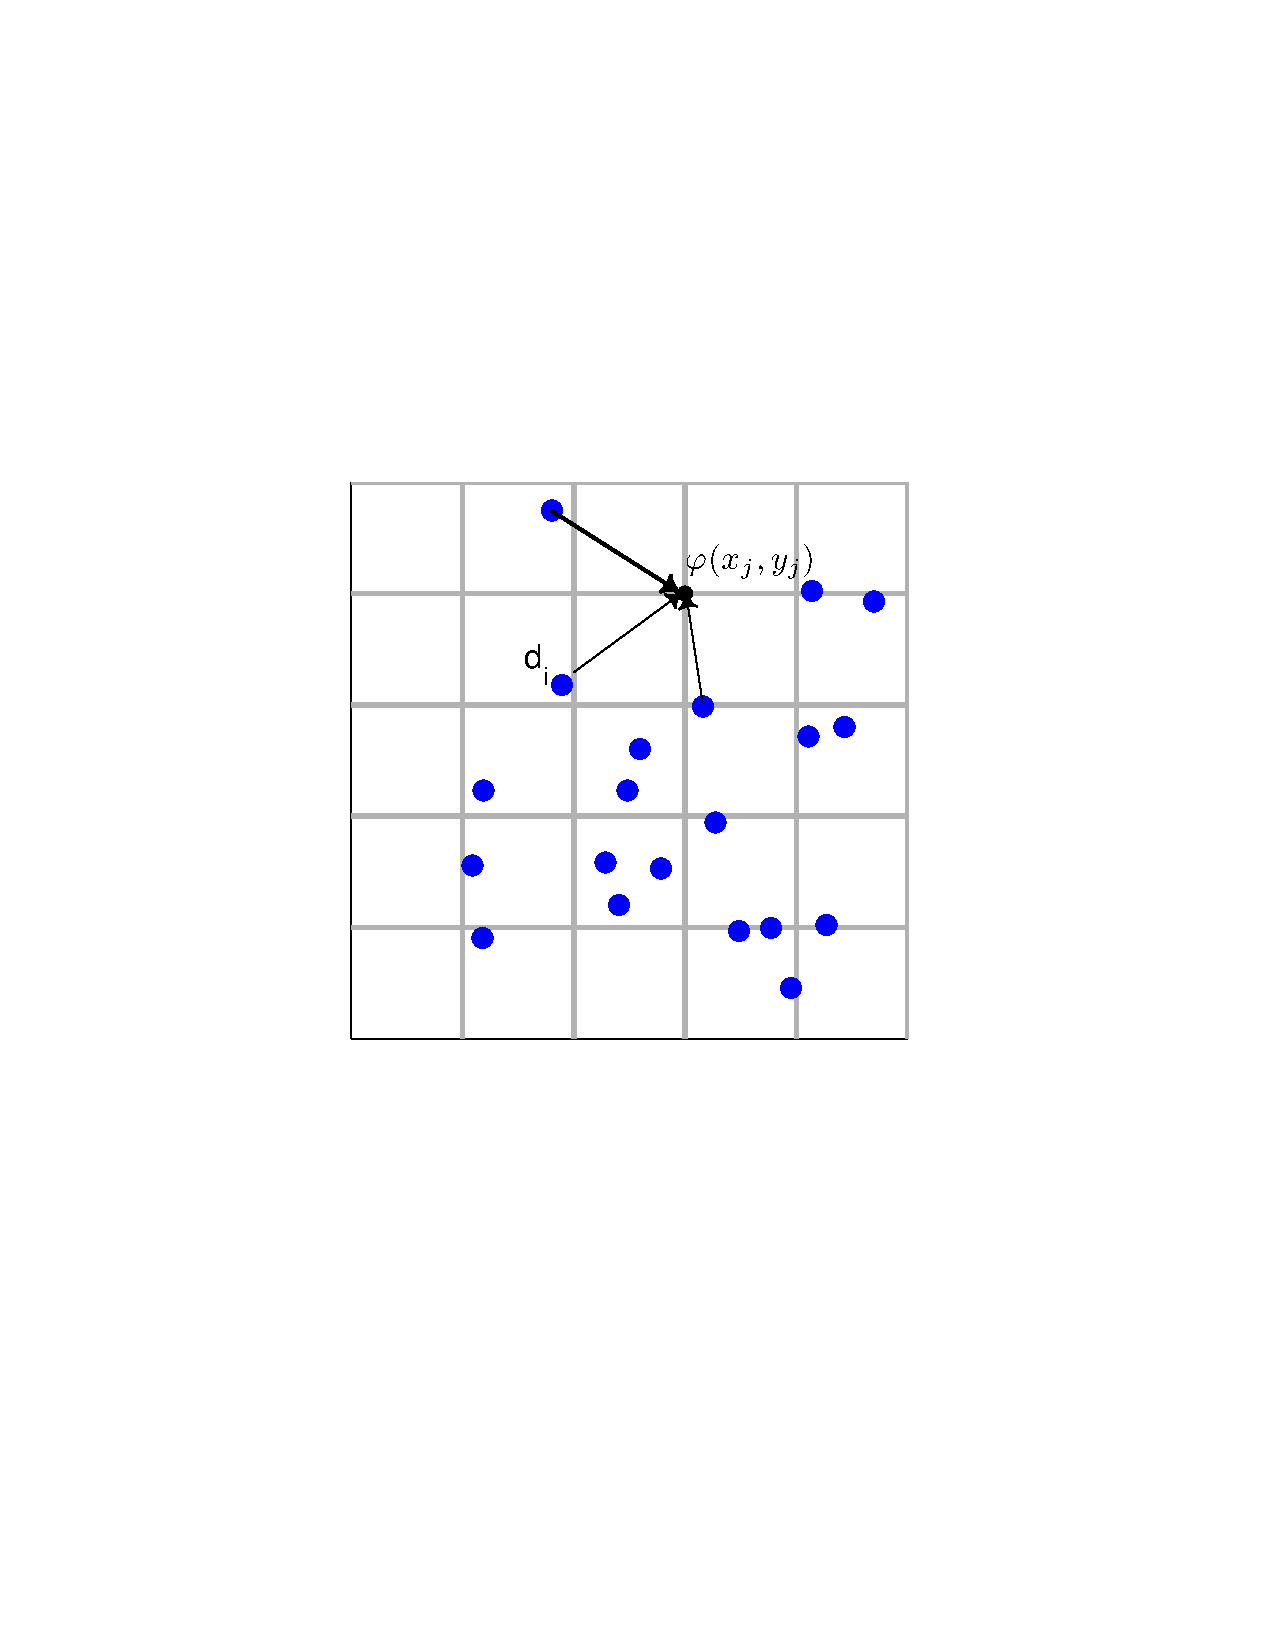
\includegraphics[width=.40\textwidth]{gridding}
		}\parbox{.5\textwidth}{
		\caption{Gridding problem: black dots indicate data positions, while the circle is the points where the field has to be determined.\label{gridproblem}}
		}
\end{figure}


\subsection{Interpolation vs. approximation}
%-------------------------------------------

When treating the gridding problem, two main techniques have to be distinguished:

\begin{enumerate}

\item \textit{Interpolation}, which implies a strict passage of the solution through the points of data. Physically, this means you assume you have no error on the data. 

% Among the methods of interpolation, let us mention: the linear, cubic, inverse distance, optimal interpolations, the \textit{kriging}, \ldots

\item \textit{Approximation} (or \textit{analysis}) provides a solution smoother than the one given by interpolation: in this case, the solution does not necessarily have to contain all the data points. The solution passes \textsl{near} the data points, so its shape is still influenced by the data. This technique allows taking into account errors on data, as well as to treat multiple data with different values at the same location. 
\end{enumerate}

\begin{figure}[htpb]
	\centering
	\parbox{.5\textwidth}{
		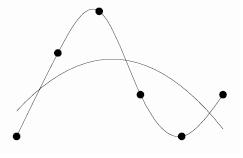
\includegraphics[width=.35\textwidth]{approx}
		}\parbox{.5\textwidth}{
		\caption{Interpolation vs. approximation.}
		}
\end{figure}


\subsection{Data analysis and gridding methodologies\label{sec:gridding}}
% ---------------------------------------------------

Because of data error and often close data points, the considered field is always reconstructed with the help of an approximation, never with a strict interpolation. 

We have to differentiate \textit{subjective} analysis, for which the way the approximation is performed is decided \textit{by hand}, and \textit{objective} analysis, which is based on predefined mathematical operations. \textit{Data assimilation} uses in addition physical/biochemical dynamic governing equations.

\textbf{Choice of a method:} among the previous methods, our choice will be the objective analysis. Indeed, the subjective analysis is not sufficiently objective, and the data assimilation depends on the region and the model.

Instead of working with the data themselves, we will work with \textit{anomalies} ($\varphi'$) with respect to a \textit{background field} ($\varphi_b$):

\begin{equation}
 \varphi(\mathbf{r}) = \varphi_b(\mathbf{r}) + \varphi'(\mathbf{r}).
 \label{background}
\end{equation}

The background field $\varphi_b$ is defined {\it a priori} and the anomalies are calculated with respect to this reference field (\textit{e.g.} climatological average, linear regression, theoretical solution). 

We assume that the anomalies can be expressed as a linear combination of the data, \textit{i.e.}

\begin{equation}
\varphi(\mathbf{r}) = \varphi_b(\mathbf{r}) + \sum_{j=1}^{N_d} w_j\, d_j,
\label{objectiveanal}
\end{equation}

where $d_{j}$ is the data anomaly at the point $\mathbf{r}= \mathbf{r_{j}}$ and $w_j$ is the relative weight of the data $j$. Now the problem consists in determining the weighting functions. 

Once the background field and the weights are known, the field can be computed at any position $\mathbf{r}$, hence gridding is possible.

From here on, we will work with anomaly only and therefore formally use $\varphi_{b}=0$.

% -------------------------------------------

\subsection{Noise on data}
% ------------------------

When measuring a field, there is always uncertainty on the value obtained (whatever the instrument and the field). \textit{Noise} does not only take into account \textit{instrumental} error (which is generally low), but also:
\begin{itemize}
\item \textit{representativeness} errors (what one measures is not always what ones intends to analyze):\\
\textit{e.g.,} skin temperature, inadequate scales, \ldots
\item \textit{synopticity} errors (when the measures are assumed to be taken at the same time):\\
\textit{e.g.,} data from a cruise \citep{RIXEN01}.
\end{itemize}

Perfect fit to data is therefore not advised. In \diva, the analysis behaviour is controlled via the \textit{signal-to-noise ratio} of data.


\section{The Optimal Interpolation method\label{sec:OImethod}}
%---------------------------------------------------------
 
The principle of \textit{Optimal interpolation} (OI hereinafter) was developed by  \cite{GANDIN65} and \cite{BRETHERTON76}. It is assumed that the true anomaly field $\varphi_t$ is one realization out of a zero mean ensemble. The problem consists in determining weights $w_j$ of Eq. (\ref{objectiveanal}), so that expected error variance of the analysis is minimal. Equation (\ref{objectiveanal}) means that the true field $\varphi_t$ we are reconstructing is decomposed into the sum of a background field $\varphi_b$ and a linear combinations of the $N_{d}$ data $d_{j}$.

Note that \textit{Kriging} \citep{KRIGE51,MATHERON63} is an equivalent technique: it uses the same criterion as OI, but with a mathematical formulation that is different. Weights $w_{i}$ are chosen from the study of the covariance between the values as a function of the distance between them.

\subsection{Mathematical formulation}
%-------------------------------------

Let us recall previous notations from section \ref{gridding} and introduce some new ones:

$\varphi$, the interpolated (or reconstructed) field,\\
$\varphi_{t}$, the true (unknown) field,\\
$\mathbf{d}$, the vector containing the $N_{d}$ data,\\
$\mathbf{r}$, the vector position.

The aim is to minimize the expected error
\begin{equation}
e^{2}(\mathbf{r}) = \overline{[\varphi(\mathbf{r})-\varphi_{t}(\mathbf{r})]^{2}}.
\end{equation}

Replacing the interpolated anomaly field by a linear combination of the data, we have 

\begin{equation}
e^{2}(\mathbf{r}) = \overline{\left[\sum_{i=1}^{N_{d}}w_{i}(\mathbf{r})d_{i}(\mathbf{r})-\varphi_{t}(\mathbf{r})\right]^{2}}.
\label{error2}
\end{equation}

We now have to determine the weights $w_{i}$ that will minimize \eqref{error2}. Let us call $\mathbf{w}(\mathbf{r})$, the vector of size $N_{d}$ containing the weights applied on the data to interpolate the field at position $\mathbf{r}$. The previous eq. is now written as 


\beqn
e^{2}(\mathbf{r}) &=& \overline{[\mathbf{w}^{T}\mathbf{d}-\varphi_{t}(\mathbf{r})]^{2}} \\
									&=& \overline{\varphi_{t}(\mathbf{r})^{2}} + \overline{\mathbf{w}^{T}\mathbf{d} \mathbf{d}^{T}\mathbf{w}} - 2 \overline{\varphi_{t}(\mathbf{r}) \mathbf{d}^{T}\mathbf{w} }
\eeqn

We define the \textit{covariance matrix}

\[
\mathbf{D} = \overline{\mathbf{d}\mathbf{d}^{T}},
\]
and the covariance of the data with respect to the real field, which is a function of $\mathbf{r}$:

\[
\mathbf{g} = \overline{\varphi_{t}(\mathbf{r})\mathbf{d}}.
\]

The expression of the error \eqref{error2} becomes, after some calculation:

\beq
e^{2}(\mathbf{r}) 
&=& \overline{\varphi_{t}(\mathbf{r})^{2}} + \mathbf{w}^{T}\mathbf{D}\mathbf{w}-2\mathbf{g}^{T}\mathbf{w} \nonumber\\
&=&  \overline{\varphi_{t}(\mathbf{r})^{2}}- \mathbf{g}^{T}\mathbf{D}^{-1}\mathbf{g}+(\mathbf{w} - \mathbf{D}^{-1}\mathbf{g})^{T}\mathbf{D}(\mathbf{w} - \mathbf{D}^{-1}\mathbf{g})
\eeq

of which the minimum is reached when

\[
\mathbf{w}=\mathbf{D}^{-1}\mathbf{g}.
\]

The corresponding error value is 

\be
\min\,e^{2}(\mathbf{r})= \overline{\varphi_{t}(\mathbf{r})^{2}}-\mathbf{g}^{T}\mathbf{D}^{-1}\mathbf{g}
\label{eq:theory_error}
\ee

and the interpolated field is computed as

\be
\varphi(\mathbf{r}) = \sum_{i=1}^{N_{d}}w_{i}(\mathbf{r})d_{i} = \mathbf{g}^{T}\mathbf{D}^{-1}\mathbf{d}.
\label{eq:theory_field}
\ee


\subsubsection{Derivation of $\mathbf{D}$ and $\mathbf{g}$}
%--------------------------------------------------------

To determine the covariance matrix, $\mathbf{D}$, and the covariance of the data with the real field, $\mathbf{g}$, the following assumptions are made: 

\begin{enumerate}
\item errors $\noise_{i}$ on measurements are not correlated, \textit{i.e.} 
\[
\overline{\noise_{i}\noise_{j}} = \noise^{2}\delta_{ij},
\]
where $\noise^{2}$ is the variance of the errors on measurement (\textit{i.e.} the noise);

\item errors on measurements are not correlated with the real field, \textit{i.e.}

\[
\overline{\noise_{i}\varphi_{t}} = 0.
\]

\end{enumerate}

With these assumptions and considering that the data at $\mathbf{r}_{i}$ is the sum of the true field at $\mathbf{r}_{i}$ and an error $\noise_{i}$, 
we deduce:

\beq
D_{ij} &=& \overline{\varphi_{t}(\mathbf{r_i})\varphi_{t}(\mathbf{r_j})}+\noise^{2}\delta_{ij} \nonumber \\
									&=& \signal^{2}\,c(\mathbf{r_i},\mathbf{r_j})+ \noise^{2}\delta_{ij},\\
 g_{i} 	&=& \overline{\varphi_{t}(\mathbf{r})d_{i}}, \nonumber \\
									&=& \signal^{2}\,c(\mathbf{r},\mathbf{r_i}), 
\eeq
where $c(\mathbf{r},\mathbf{r_i})$ is the \textit{correlation function} and $\signal$ is the \textit{signal} of the data.



\section[VIM and its implementation]{VIM and its implementation \diva}
% ---------------------------------------

VIM stands for \textit{Variational Inverse Method}. This method was initially designed for climatology: in that case, you have generally high resolution vertical profiles, sufficient profiles in all seasons, but irregular horizontal coverage \citep{BRASSEUR96}. Thus a spatial analysis on horizontal planes is needed. 

Relatively large number of data points in each plane penalizes Optimal Interpolation (OI) methods, because these methods require the inversion of a $N_{d}$-by-$N_{d}$ matrix, \textit{i.e.} a number of operations proportional to $N_{d}^{3}$ (see Tab. \ref{tabdata} and eq. \ref{eq:theory_error}).

This is the reason why VIM resorts to the expertise in efficient finite-element solvers.

\diva\, stands for \textit{Data-Interpolating Variational Analysis} and is the implementation of VIM. It is designed to solve 2-D differential or variational problems of elliptic type with a finite element method.


\subsection{Formulation\label{sec:formulation}}
% ----------------------

We are looking for the field $\varphi$ which minimizes the variational principle:

\begin{equation}
J \left[\varphi\right] =\sum_{j=1}^{Nd}\mu_{j}\left[d_{j}-\varphi(x_{j},y_{j})\right]^{2}+
\| \varphi\| ^{2}
\label{divaformula}
\end{equation}

with
\begin{equation}
\|\varphi\|=\int_{D}(
\alpha_{2} 
\nablab\nablab\varphi : \nablab\nablab\varphi +\alpha_{1}
\nablab\varphi \cdot \nablab\varphi + \alpha_{0} \varphi^{2})\, d D
\label{divaformula2}
\end{equation}

where
\begin{itemize}
\item
$\alpha_0$ penalizes the field itself (anomalies),
\item
$\alpha_1$ penalizes gradients (no trends),
\item 
$\alpha_2$ penalizes variability (regularization),
\item 
$\mu$ penalizes data-analysis misfits (objective).
\end{itemize}
Without loss of generality we can chose $\alpha_2=1$ (homogeneous function \ref{divaformula}).



\subsubsection{Parameters meaning\label{sec:parammeaning}}
% --------------------------------------------------------

Writing Eq. (\ref{divaformula}) and (\ref{divaformula2}) in non-dimensional form (with $\frac{1}{L}\tilde{\nablab}=\nablab$, $L$ being a characteristic length of the problem), we have

\begin{equation}
J[\varphi]=\sum_{j=1}^{Nd}\mu[d_{j}-\varphi(x_{j},y_{j})]^{2}+
 \int_{\tilde{D}}\left(
\frac{1}{L^4} \tilde{\nablab}\tilde{\nablab}\varphi : \tilde{\nablab}\tilde{\nablab}\varphi + \frac{\alpha_{1}}{L^2}
\tilde{\nablab}\varphi \cdot \tilde{\nablab}\varphi + \alpha_{0} \varphi^{2} \right) L^2\,d\tilde{D}
\end{equation}
and multiplying by $L^{2}$:
\begin{equation}
{J}[\varphi]=\sum_{j=1}^{Nd}\mu L^2 [d_{j}-\varphi(x_{j},y_{j})]^{2}+
 \int_{\tilde{D}}\left(
 \tilde{\nablab}\tilde{\nablab}\varphi : \tilde{\nablab}\tilde{\nablab}\varphi + { \alpha_{1} L^2}
\tilde{\nablab}\varphi \cdot \tilde{\nablab}\varphi + \alpha_{0} L^4 \varphi^{2} \right) \,d\tilde{D}
\label{divaformulaadim}
\end{equation}


Hence $\alpha_0$ fixes the length scale over which variations are significant to move the \hyperlink{KERNEL}{\textit{kernel function}} of the norm from one to zero:
\begin{equation}
\alpha_0 L^4 = 1
\end{equation}
$ \mu L^2$ fixes the relative weight on data (signal, $\sigma^2$) versus regularization (noise, $\epsilon^2$):
\begin{equation}
\mu L^2= 4 \pi \frac{\sigma^2}{\epsilon^2}= 4 \pi S/N 
\label{defmu}
\end{equation}

Finally  $\alpha_1$ fixes the influence of gradients:

\begin{equation}
\alpha_1 L^2 = 2 \xi
\end{equation}
where   $\xi=1$ if penalization on the gradients is enforced, $\xi=0$ if no penalization is enforced. $\xi$ is a non-dimensional parameter close to one if the gradients are to be penalized with a similar weight than the second derivatives.


\subsubsection{Weights on data}
% -----------------------------

A weight $\mu_i$ can be assigned to each data $d_i$. This weight expresses the confidence you have in a particular data. It is expressed as a function of the signal-to-noise ratio and the correlation length \cite{BRANKART96}: 

\begin{equation}
\mu=\frac{\sigma^{2}}{\epsilon^{2}} \frac{4 \pi}{L^{2}}
\end{equation}


when $\xi=1$. In  \diva, the fourth column of the data input file, if present, allows one 
to apply a different relative weight to each point. 


\subsubsection{Background field\label{sec:backgroundfield}}
% ---------------------------------------------------------

Normally, interpolation (and extrapolation) works on anomalies with respect to a background field (Eq. \ref{background}). \diva\, allows you to work with different background fields:

\begin{itemize}
\item no treatment is applied (the data you treat are already anomalies);
\item the mean of data is subtracted from the data values;
\item the linear regression (plane) is subtracted;
\item additional subtracted semi-normed field ($\alpha_0=0$ and large $L$) obtained by two chained \diva\, executions. Matrix K is decomposed into a norm-related term and a data related term.
\end{itemize}

In particular when no treatment is applied (with $\alpha_0 > 0$), the minimization forces the analysis toward zero when there are no
data points in a distance comparable to $L$. This is coherent with the idea of an anomaly only.

\subsection{Resolution by Finite-Element Method}
% ----------------------------------------------

Minimization of (\ref{divaformula}) is actually performed by a Finite-Element Method (FEM), hence the need for generating a finite-element grid. 
Because the field to analyse is only defined in the water, the minimization also works only within the contours defining the coastline or more generally, the considered isobath.

Thus the grid generation has to be consistent with the coasts existing in the considered region. The corresponding mathematical problem is referred to the \textit{Constrained Triangulation}. %More details about the FEM will be given in section \ref{femgrid}.


To solve Eq. (\ref{divaformula}), the real domain is split into a mesh of $N_e$ finite elements:

\be
J[\varphi] = \sum_{e=1}^{N_{e}}J_{e}(\varphi_{e}).
\label{eq:split}
\ee

In each element the solution is a combination of shape functions (3$^{rd}$ order polynomials) and the continuity between elements is assured by identification of adjacent \textit{connectors}:

\be
\varphi_{e}(\mathbf{r_e})=\mathbf{q_e}^{T}\mathbf{s}(\mathbf{r_e}),
\label{eq:connectors}
\ee
with $\mathbf{q}$, the connectors (our new unknowns),\\
\hphantom{with} $\mathbf{r_e}$, the position in a local coordinate system.

Substituting \eqref{eq:connectors} in \eqref{eq:split} and using the variational principle \eqref{divaformula}, we get

\be
J_{e}(\mathbf{q_e}) = \mathbf{q_e}^{T}\mathbf{K_e}\mathbf{q_e}-2\mathbf{q_e}^{T} \mathbf{g_{e}}+\sum_{i=1}^{N_{d_{e}}}\mu_{i}d_{i}
\label{eq:elements}
\ee
where $\mathbf{K_e}$ is the \textit{local stiffness} matrix and\\
\hphantom{where} $\mathbf{g}$ is a vector which depends on local data.

On the whole domain, \eqref{eq:elements} reads

\be
J(\mathbf{q}) = \mathbf{q}^{T}\mathbf{K}\mathbf{q}-2\mathbf{q_e}^{T} \mathbf{g_{e}}+\sum_{i=1}^{N_{d}}\mu_{i}d_{i},
\label{eq:domain}
\ee
of which the minimum is reached when

\be
\mathbf{q}=\mathbf{K}^{-1}\mathbf{g}.
\label{eq:solution}
\ee
Matrix $\mathbf{K}$ has a size approximatively proportional to the number of degrees of freedom of the system, but can be very sparse if the elements are properly sorted. In that case the number of operations to invert it is approximatively proportional to the power $5/2$ of the number of degrees of freedom.

To map the data on the finite element mesh, a transfer operator $\mathbf{T_{2}}$ (depending on the shape functions) is applied:

\[\mathbf{g}=\mathbf{T_2}(\mathbf{r})\mathbf{d},\]

and to have the solution at any location inside the domain, another transfer $\mathbf{T_{1}}$ is applied:

\[\boldsymbol{\varphi}(\mathbf{r})=\mathbf{T_1}(\mathbf{r})\mathbf{q}.\]

Combining the two previous equations, we obtain the relation between $\varphi$, the interpolated field at location $\mathbf{r}$,  and the data vector $\mathbf{d}$:

\be
\boldsymbol{\varphi} = \mathbf{T_1}(\mathbf{r})\mathbf{K}^{-1}\mathbf{T_2}(\mathbf{r}) \mathbf{d}.
\label{eq:solution2}
\ee


\subsection{Error field}
% ----------------------

For any analysis method, a quantification of associated errors is an essential feature, since it gives the user an indication of the reliability of the results. Broadly speaking we may expect the error field to be affected by:
\begin{enumerate}
\item the data coverage: the error field is expected to be higher where the data coverage is lower;
\item the noise on the data: the more imprecision we have on the data, the higher will be the error field.
\end{enumerate}

We will see in the next sections how \diva\, computes this error field.

\subsubsection{Derivation of the error field}
%--------------------------------------------

Optimal Interpolation (Sec. \ref{sec:OImethod}) allows the simultaneous derivation of analysis and error fields, but is not adapted for large data sets, while the spline methods are suitable for large amount of data but does not offer an error estimation.

To fill in this gap, \cite{BRANKART98} and \cite{RIXEN00} proposed a heuristic statistical error expression for the VIM: in \diva, error fields are calculated by analogy with OI: since analysis in OI is equivalent to analysis with VIM \footnote{Insofar as the reproducing Kernel of VIM and the covariance function of OI are identical.} and 
since error field of OI equals analysis of covariance fields, error field of VIM equals analysis (by VIM) of covariance fields.

Mathematically, according to the developments of section \ref{sec:OImethod}, we have:

\begin{tabular}{rlccrl}
\hline
\rule{0pt}{4ex}Solution &OI:  & $\varphi(\mathbf{r})$ &=& $\underbrace{\mathbf{g}(\mathbf{r})^{T}\mathbf{D}^{-1}}_{(\star)}$				&$\mathbf{d}$\\
\rule{0pt}{4ex}Solution				 &VIM:	& $\varphi(\mathbf{r})$ &=& $\underbrace{\mathbf{T_{1}}(\mathbf{r})\mathbf{K}^{-1} \mathbf{T_{2}}(\mathbf{r})}_{(\star\star)}$	&$\mathbf{d}$\\
\rule{0pt}{4ex}Error		 &OI:  & $e^{2}(\mathbf{r})$   &=& $\epsilon^{2}(\mathbf{r})-\underbrace{\mathbf{g}(\mathbf{r})^{T}\mathbf{D}^{-1}}_{(\star)}$		&$\mathbf{g}(\mathbf{r})$	\\		
				\hline
\rule{0pt}{4ex}$\stackrel{\textrm{by analogy}}{\rightarrow}$				 &VIM:	& $e^{2}(\mathbf{r})$   &=& $\epsilon^{2}(\mathbf{r})-\underbrace{\mathbf{T_{1}}(\mathbf{r})\mathbf{K}^{-1} \mathbf{T_{2}}(\mathbf{r})}_{(\star\star)}$&$\mathbf{g}(\mathbf{r})$\\
\hline
\end{tabular}



In practice, the data input of the analysis tool for an error calculation is a vector containing the
covariance of data points with the point in which the error estimate is to be calculated. 

The problem is now how to specify this vector $\mathbf{g}$. 


\subsection{Kernel and correlation function \label{sec:kernel}}
% ------------------------------------------

\hypertarget{KERNEL}{Kernel} functions can be examined by analyzing a single point with high signal-to-noise ratio and no background field (Fig. \ref{singleanalysis}). In this particular case, we performed an analysis with a point located at the center $(0,0)$ of a square domain. The correlation length is equal to $1$ and the signal-to-noise ratio is taken equal to $1000$.

The exact function in an infinite domain is given by 

\begin{equation}
K(r)=\left(\frac{r}{L}\right)K_{1}\left(\frac{r}{L}\right),
\label{kernelfunction}
\end{equation}

where $r$ is the Euclidean distance,\\ 
\hphantom{where} $L$ is the correlation length and \\
\hphantom{where} $K_{1}$ is the modified Bessel function \citep[][page 359]{ABRAMOWITZ64}.

%\footnote{The \textit{modified Bessel's equation} is the differential equation of order 1. 
%
%\begin{equation}
%z^{2}\frac{d^{2}y}{dz^{2}}+z\frac{dy}{dz}-(z^{2}+\nu^{2})y=0, 
%\label{besselmodif}
%\end{equation}
%
%where $\nu$ is a real constant. The solutions of this equation are called the \textit{modified Bessel functions}. A solution of the second kind of \eqref{besselmodif} is $K_{\nu}(z)$, defined by 
%
%\[K_{\nu}(z)=\left(\frac{\pi}{2}\right)^{\nu}\frac{I_{-\nu}(z)-I_{\nu}(z)}{\sin(\nu\pi)},\]
%
%where $I_{\nu}(z)$ and $I_{-\nu}(z)$ form a fundamental set of solutions of \eqref{besselmodif} for non integer $\nu$:
%
%\[I_{\nu}(z)=\left(\frac{z}{2}\right)^{\nu}\sum_{k=0}^{+\infty}\frac{\left(\frac{z^{2}}{4}\right)^{k}}{k!\,\Gamma(\nu+k+1)},\]
%
%and $\Gamma(a)$ is the \textit{gamma function}.  \\
%
%\underline{Source}: \matlab\, Help for function \texttt{besselk}.} 

The choice of this correlation model results from the mathematical structure of the variational method \citep{BRASSEUR96}.

Fig. \ref{kernel1} shows both the exact solution (\ref{kernelfunction}) and the correlation function by a single point analysis. The two curves are close to each other, the differences between the two curves being only due to the boundaries.

In an infinite domain, the correlation function was shown to be proportional to the Kernel of the VIM norm.

\begin{figure}[H]
\centering
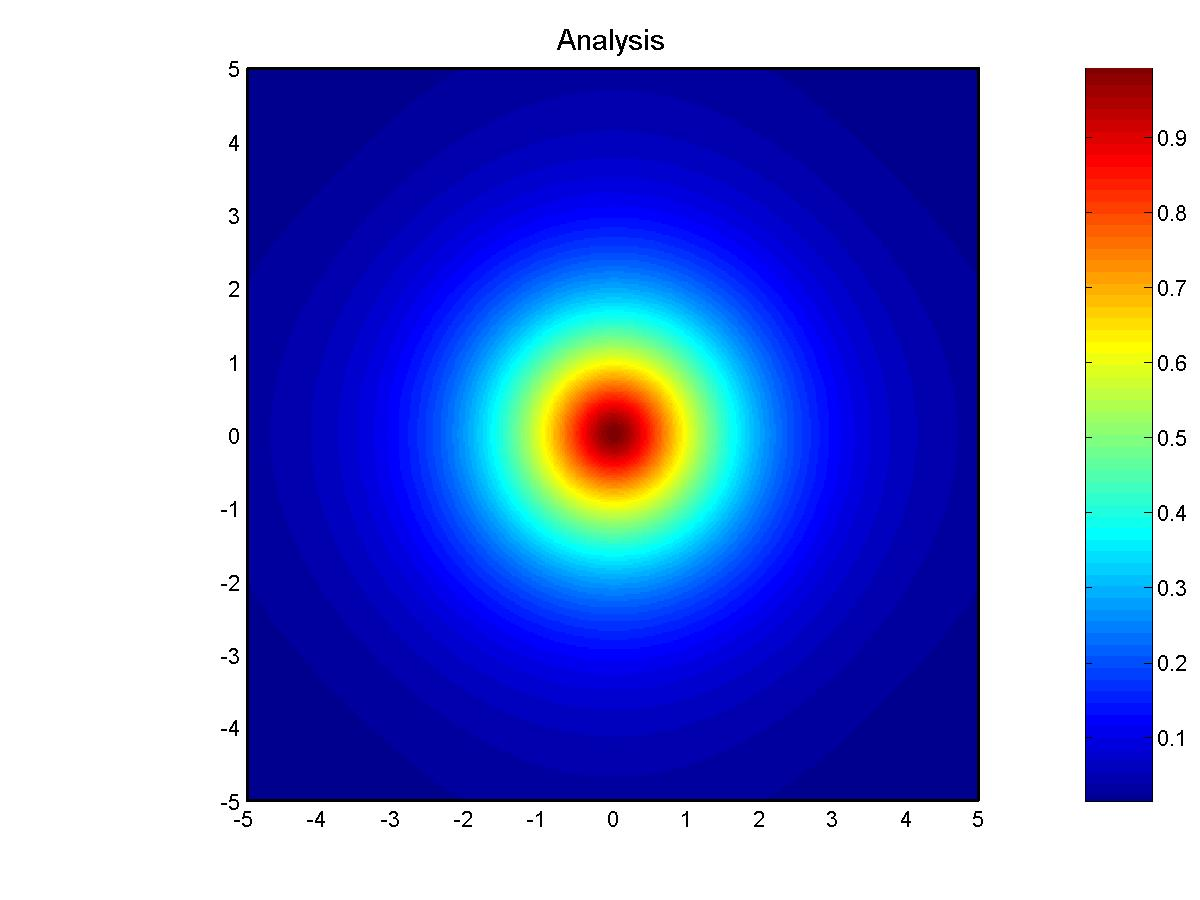
\includegraphics[width=.75\textwidth]{singlepointanalysis}
\caption{Analysis of a single data point with high signal-to-noise ration and no background field.\label{singleanalysis}}
\end{figure}

\begin{figure}[H]
\centering
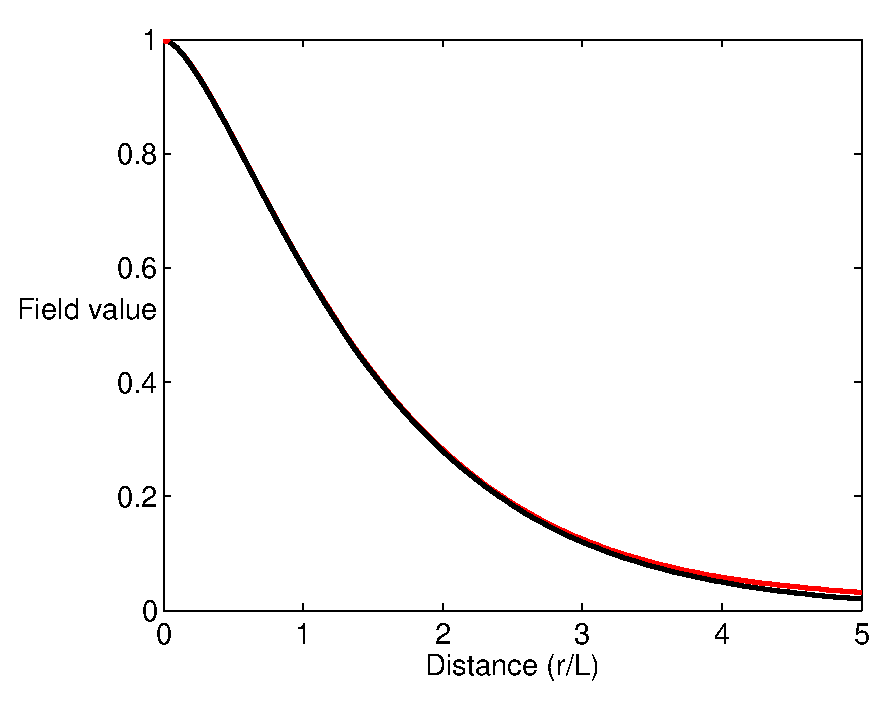
\includegraphics[width=.75\textwidth]{kernelf}
\caption{Kernel function is given in red, while the blue curve comes from the analysis of a single point.\label{kernel1}}
\end{figure}


The Kernel function can be used to calibrate \diva\, parameters ($\alpha_0, \alpha_1, \mu$) so as to fit observed covariance functions. This principle is used by the tool \texttt{divafit} which helps one to estimate the correlation length (see Sec. \ref{sec:divafit}).

It can also be used for specifying the covariance for error calculations.% (Sec. \ref{}).



\section{Comparison between the methods}
%---------------------------------------

Numerous methods are available for data interpolating. Tab. \ref{tabdata} shows different characteristics of each methods: error minimization ($\min( \varepsilon^2)$), extension to 3D, multivariate analysis, number of operations, error estimate ($\varepsilon(\mathbf{r})$), \textit{a priori} known parameters, control parameters and treatment of anisotropy. 


\begin{table}[htpb]
\begin{flushleft}
\caption{Characteristics of different methods of data analysis. \label{tabdata}}
\begin{tabular}{lcccccccc}
\hline
Method   & $\min( \varepsilon^2)$ & 3D       & Multivar & Ops/image        & $ \varepsilon(\mathbf{r})$& \textit{a priori}& C.V. & anis. \\ 
\hline
Cressman &                    & $\star$  &  $\star$ & $N_d N_a$        &                        & $w(r/L)$         &($L$) & ($\star$)  \\ 
OI     &   $\star$          & $\star$  &  $\star$ & $N_d^3+ N_d N_a$ &  $\star$               & $c(r/L)$         & $L,\sigma^2/\mu^2$&($\star$)\\ 
{\bf VIM}&   $\star$       & ($\star$)& ($\star$)& $N_a^{5/2}$      &  $\star$               & $K(r/L)$         & $L,\sigma^2/\mu^2$&($\star$)\\
\dineof\footnote{described in Sec. \ref{lasttool}.}   &   ($\star$)        &  $\star$ &  $\star$ & $N_a^{5/4}$      &  ($\star$)   &  stat.          & $N$               & $\star$\\ 
\hline
\end{tabular}
\end{flushleft}
\end{table}
\clearpage

where 
\begin{itemize}
\item[$N_d$]: number of data points,
\item[$N_a$]: number of grid points for analysis,
\item[$N$]: number of EOFs,
\item[$L$]: correlation length,
\item[$\sigma^2/ \varepsilon^2$]: signal to noise ratio,
\item[$\star$]: available feature,
\item[($\star$)]: available with some adaptations.
\end{itemize}

\subsection{Drawbacks of OI}
%-----------------------------------

The first inconvenient is that OI is not well-adapted for situations where the number of data to treat is large, since inverting the correlation matrix requires  $\mathcal{O}(N_{d}^{3})$ operations. Typically VIM analysis (error) becomes faster than OA when more than 250 (130) data are available \citep{RIXEN00}. 

A second important factor is the propagation of information through islands and continents when working with OI: as the correlation functions are isotropic, the method cannot take into account spatial anisotropies due to boundaries, whereas VIM only covers the real domain and therefore detects automatically obstacles. 

Finally, although OI provides the best analysis in the sense that it gives the minimum expected error, the method has the drawback of not being objective: the covariance of the unknown field, and the standard deviation of observational errors generally have to be chosen subjectively by he user.

%Basic examples in section \ref{testcases} will illustrate the differences between analysis fields provided by OI and by VIM.


\subsection{OI vs. VIM}
%-----------------------------------------

\cite{RIXEN00} compared the two methods by testing quasi-synoptic salinity data. Results showed that the main differences between OA and VIM occur in coastal areas and around islands ($\mathcal{O}(0.10)$), whereas the differences range from $-0.01$ to $0.02$ within the domain. The same conclusions were drawn when they compared OI and VIM in the case of climatological data set: both fields were nearly identical, except in the vicinity of the coasts (differences of up to 0.1).

A summary of the main characteristics of the two methods is found in Tab. \ref{tabOAVIM}.


\begin{table}[H]
\begin{flushleft}
\caption{Statistical equivalence between OI and VIM (from \cite{RIXEN00})\label{tabOAVIM}}
\begin{tabular}{lll}
\hline
											&		OI																																										  	&VIM \\
											\hline
Minimization \rule{0pt}{3ex}& $e^{2}(\mathbf{r})= \overline{ [\varphi(\mathbf{r})-\varphi_{t}(\mathbf{r})]^{2}}$					& $J[\varphi]=\sum_{i=1}^{N_d}\mu_{i}[d_{i}-\phi(\mathbf{r_{i}})]^{2}+\left\|\varphi\right\|^{2}$\\
Solution							& $\varphi(\mathbf{r})= \mathbf{c}^{T}(\mathbf{r})\mathbf{D}^{-1}\mathbf{d}$								& $\varphi(\mathbf{r})= \mathbf{c}^{T}(\mathbf{r})\mathbf{D}^{-1}\mathbf{d}$	\\
Data correlation			& $[\mathbf{D}]_{ij}=\signal^{2} c(\mathbf{r_{i}},\mathbf{r_{j}})+\noise^{2}\delta_{ij}$	& $[\mathbf{D}]_{ij}=K(\mathbf{r_i},\mathbf{r_j})+(1/\mu)\delta_{ij}$\\
Data-field covariance & $[\mathbf{c}]_{i}=\signal^{2} c(\mathbf{r},\mathbf{r_{i}})$																						& $[\mathbf{c}]_{i}=K(\mathbf{r},\mathbf{r_{i}})$	\\
\hline
\end{tabular}
\end{flushleft}
\end{table}


 
 
 
 
 
 
 

\section{Additional tools}
% ------------------------

\diva\, software is provided with addition tools designed for parameters adjustment and validation of results.


\subsection{Generalized Cross Validation (GCV)\label{firsttool}}
%---------------------------------------------------------------

GCV allows estimating global errors and calibration of the correlation length $L$ and the signal-to-noise ratio $\snr=\frac{\signal^{2}}{\noise^{2}}$.
The method consists in setting one or several data aside and perform an analysis in order to obtain a global error estimate. GCV applies analysis to random anomalies at the same locations as real data. A detailed description of the method is provided in Chap. \ref{gcv}.

 
\subsection{Advection constraint}
%--------------------------------


The advection constraint aims at taking into account the transport of information (temperature, salinity, or any other tracer) by the velocity field. 
This is the topic of Chap. \ref{chap:advection}


\subsection{Three-dimensional analysis}
%--------------------------------------

\diva\, is able to carry out analysis in oceanic basin, by applying successive analysis on horizontal layers, from surface to bottom. A set of scripts (\texttt{diva3D*}) are designed to perform such analysis in an automatic way.

The whole procedure is described in the second volume of the manual.

\subsection{Static instabilities removal}
%----------------------------------------

The reconstruction of three-dimensional fields of temperature and salinity by stacking of layers of analysed fields may leads to unstable density fields. A procedure implemented in \diva\, in order to remove these instabilities is presented in the second volume of the manual.

\subsection{\dineof\label{lasttool}}
%-----------------------------------

\hypertarget{DINEOF}{\dineof}\, stands for \textit{Data INterpolating Empirical Orthogonal Function}.

It is designed to exploit repeated observations with missing data (\textit{e.g.} a series of collocated satellite images with clouds).
For more details about \dineof, the reader is invited to consult:
\cite{ALVERA05,ALVERA07,BECKERS03,BECKERS06}, \url{http://modb.oce.ulg.ac.be/mediawiki/index.php/DINEOF} and   \url{http://ocgmod2.marine.usf.edu/DINEOF-welcome.html}.



\subsection{Future developments}
%--------------------------------

Some aspects of \diva\, are still under development. Improvements in progress are:

\begin{itemize}
%\item 3D extensions: from surface to deep layers through EOF calculated from data set (\dineof\, approach), and application in horizontal planes.
%\item Static stability constraints.
\item Multivariate approaches (easy in OI, but more difficult in VIM).
\item Parameter calibration by cross validation in multivariate version.
\item Data query modules, possibly through ODV.
\item Strategy for combined analysis of satellite and {\it in situ} data.
\end{itemize}

